% Progress report against the supervisor's requirements (Robotic-Manipulation-v1-requirement-supervisor.pdf).
% Build: pdflatex progress_report.tex (twice). Figures: .venv/bin/python docs/report/make_figures.py
\documentclass[10pt,a4paper]{article}
\usepackage[margin=2cm]{geometry}
\usepackage[T1]{fontenc}
\usepackage{lmodern}
\usepackage{microtype}
\usepackage{graphicx}
\usepackage{booktabs}
\usepackage{tabularx}
\usepackage{array}
\usepackage{xcolor}
\usepackage{tikz}
\usetikzlibrary{positioning,arrows.meta,fit,calc}
\usepackage{float}
\usepackage{caption}
\usepackage{subcaption}
\usepackage{enumitem}
\usepackage{amsmath}
\usepackage[hidelinks]{hyperref}

\definecolor{good}{HTML}{0CA30C}
\definecolor{warn}{HTML}{C98500}
\definecolor{crit}{HTML}{D03B3B}
\definecolor{sOne}{HTML}{2A78D6}
\definecolor{inktwo}{HTML}{4E5157}
\newcommand{\met}{\textcolor{good}{\textbf{Met}}}
\newcommand{\partmet}{\textcolor{warn}{\textbf{Partly met}}}
\newcommand{\notmet}{\textcolor{crit}{\textbf{Not met}}}
\newcommand{\figdir}{figs}
\captionsetup{font=small,labelfont=bf,skip=4pt}
\setlist{nosep,leftmargin=1.2em}
\setlength{\parindent}{0pt}
\setlength{\parskip}{4pt}
\renewcommand{\arraystretch}{1.15}

\title{\vspace{-1.2cm}POGS Re-implementation:\\Progress Against the Project Requirements}
\author{[Student name] \quad Supervisor: [Supervisor name]}
\date{23 November 2026}

\begin{document}
\maketitle
\vspace{-0.6cm}

\begin{center}
\small Simulation only. One trained Gaussian splat per scene. NVIDIA RTX 4070 (12\,GB). Code: branch \texttt{research-plan-rev2}.
\end{center}

%==========================================================================
\section*{Summary}
\begin{table}[H]
\centering\small
\begin{tabularx}{\linewidth}{@{}l X l X l l@{}}
\toprule
& Requirement & Target & Result & Status & Sec.\\
\midrule
R1 & Object grouping: splats with and without one object & check & Object Gaussians isolated; IoU 0.76 to 0.98 (5 objects) & \met & \ref{sec:r1}\\
R2 & Project structure; Python 3.12, CUDA 13.0, PyTorch 2.14, torchmetrics & layout & As specified; 57 tests pass & \met & \ref{sec:r2}\\
R3 & Tool perturbation, step-wise to $30^\circ$ and back; splats, pose, KL & $30^\circ$ & 15/15 recovered; rotation error at $y$ 1.4 to $1.7^\circ$ & \met & \ref{sec:r3}\\
R4 & In-grasp perturbation recovery rate & 80\% & 4 to 28\% (strict rule); 34 to 78\% (paper's rule) & \notmet & \ref{sec:r4}\\
R5 & Latency of each 2D foundation model & table & 8 of 11 measured (one on an earlier stack) & \partmet & \ref{sec:r5}\\
R6 & Tracking frequency & 5\,Hz & 5.7\,Hz at 100\% ADD-S in one setting (3 seeds) & \partmet & \ref{sec:r6}\\
\bottomrule
\end{tabularx}
\end{table}

Beyond the requirements, Section~\ref{sec:further} identifies why R4 is not met: a systematic roll error about the drill bit, caused by a mechanism in the DINO feature loss.

\paragraph{Definitions.} \emph{Recovered}: tool-tip error $<3$\,cm and rotation error $<5^\circ$; in R4 ten frames (2\,s) after the perturbation and never lost afterwards, in R3 at the final state $y$. \emph{Paper's rule}: as recovered, but rotation about the drill-bit axis is left free, as in POGS Sec.~V-B. \emph{KL}: opacity-weighted Kullback--Leibler divergence between two sets of 3D Gaussians. \emph{Static}: a baseline that never moves; it is included in every comparison as a null model.

%==========================================================================
\section{R1: Object grouping features}\label{sec:r1}
\begin{figure}[H]
\centering
\begin{subfigure}[b]{0.56\linewidth}\centering
\includegraphics[width=\linewidth]{\figdir/o1_renders.jpg}
\caption{Columns: ground truth, full splat, splat \emph{without} the object, splat with \emph{only} the object. Rows: mustard bottle, soup can, mug, apple, cereal box.}
\end{subfigure}\hfill
\begin{subfigure}[b]{0.42\linewidth}\centering
\includegraphics[width=\linewidth]{\figdir/o1_grouping_scores.pdf}
\caption{Overlap of each object's Gaussian group with ground truth (35 views).}
\end{subfigure}
\caption{Removing one group deletes exactly that object; rendering the group alone shows only that object. The soup can is the weakest group (recall 0.65; some can Gaussians remain in the scene).}
\end{figure}

%==========================================================================
\section{R2: Project structure and environment}\label{sec:r2}
\begin{figure}[H]
\centering
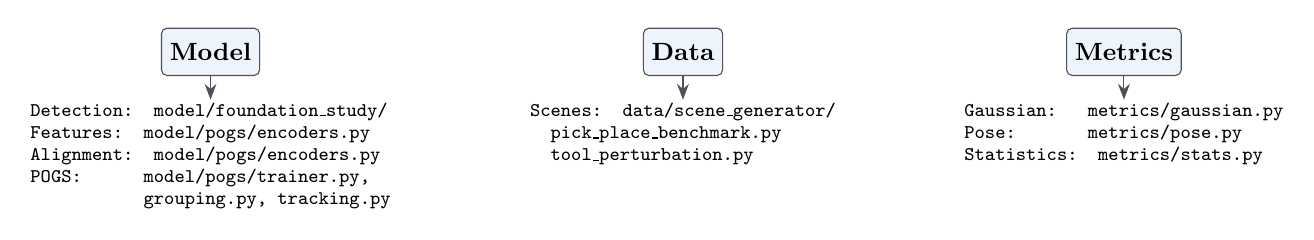
\begin{tikzpicture}[font=\small,
  grp/.style={draw=inktwo,rounded corners=2pt,fill=sOne!8,minimum height=6mm,inner sep=3pt},
  leaf/.style={align=left,font=\scriptsize\ttfamily,inner sep=1pt},
  ar/.style={-{Stealth[length=2mm]},draw=inktwo}]
\node[grp] (m) at (0,0) {\textbf{Model}};
\node[grp] (d) at (6.0,0) {\textbf{Data}};
\node[grp] (me) at (11.6,0) {\textbf{Metrics}};
\node[leaf,below=3mm of m,anchor=north] (ml) {%
Detection: model/foundation\_study/\\
Features:\ \ model/pogs/encoders.py\\
Alignment: model/pogs/encoders.py\\
POGS:\ \ \ \ \ \ model/pogs/trainer.py,\\
\ \ \ \ \ \ \ \ \ \ \ grouping.py, tracking.py};
\node[leaf,below=3mm of d,anchor=north] (dl) {%
Scenes: data/scene\_generator/\\
\ \ pick\_place\_benchmark.py\\
\ \ tool\_perturbation.py};
\node[leaf,below=3mm of me,anchor=north] (mel) {%
Gaussian:\ \ \ metrics/gaussian.py\\Pose:\ \ \ \ \ \ \ metrics/pose.py\\Statistics: metrics/stats.py};
\draw[ar] (m) -- (ml); \draw[ar] (d) -- (dl); \draw[ar] (me) -- (mel);
\end{tikzpicture}
\caption{Repository layout mapped to the requested structure.}
\end{figure}
\vspace{-2mm}
\begin{center}\small
\begin{tabular}{@{}lllllr@{}}
\toprule
Python & CUDA & PyTorch & torchmetrics & gsplat & Tests\\
\midrule
3.12.16 & 13.0 & 2.14.1+cu130 & 1.9.0 & 1.5.3 & 57 passed, 1 skipped\\
\bottomrule
\end{tabular}
\end{center}

%==========================================================================
\section{R3: Tool perturbation recovery to \texorpdfstring{$30^\circ$}{30 degrees}}\label{sec:r3}
Protocol as specified: splats $x$ at rest; rotate the drill in $+5^\circ$ (or $+10^\circ$, $+15^\circ$) steps to $30^\circ$ (state $p$); rotate back in equal steps to the original orientation (state $y$); compare $y$ with $x$ for splats and pose. Five trajectories per step size.

\begin{figure}[H]
\centering
\begin{subfigure}[b]{0.49\linewidth}\centering
\includegraphics[width=\linewidth]{\figdir/o3_step_trace.pdf}
\caption{$5^\circ$ steps: commanded angle (top) and rotation error (bottom; mean and range over 5 trials).}
\end{subfigure}\hfill
\begin{subfigure}[b]{0.49\linewidth}\centering
\includegraphics[width=\linewidth]{\figdir/o3_jumps.pdf}
\caption{Additional test: a single jump. Recovery holds up to $60^\circ$; at $90^\circ$ the tip error grows to $5.3\pm10.4$\,cm.}
\end{subfigure}
\caption{POGS follows the step sequence with less than $5^\circ$ error throughout. Static fails because each trial first moves the drill to a random start pose.}
\end{figure}

\begin{table}[H]
\centering\small
\begin{tabular}{@{}l l c c c c c@{}}
\toprule
Step & Method & Recovered & Rot.\ error at $y$ & Tip error at $y$ & KL$(x\,\|\,y)$ & KL(GT $\|$ tracked) at $y$\\
\midrule
$5^\circ$  & POGS   & 5/5 & $1.4^\circ$ & 0.63\,cm & 0.40 & 32\\
$10^\circ$ & POGS   & 5/5 & $1.7^\circ$ & 0.60\,cm & 0.20 & 32\\
$15^\circ$ & POGS   & 5/5 & $1.7^\circ$ & 0.56\,cm & 0.34 & 32\\
all        & Static & 0/5 & $29.5^\circ$ & 8.66\,cm & 0 & 1478\\
\bottomrule
\end{tabular}
\caption{Splats and pose at $y$ compared with $x$. KL$(x\|y)$ alone is not a recovery test: a tracker that never moves scores 0. It is therefore reported together with the KL to the ground-truth splat and the pose error.}
\end{table}

%==========================================================================
\section{R4: In-grasp tool perturbation recovery rate}\label{sec:r4}
The drill is grasped, lifted and held; it is then rotated in the gripper by $\pm15^\circ$ or $\pm30^\circ$ about the grasp axis. Fifty trials per setting.

\begin{figure}[H]
\centering
\begin{subfigure}[b]{0.49\linewidth}\centering
\includegraphics[width=\linewidth]{\figdir/o4_recovery.pdf}
\caption{Recovered trials. The paper reports 48/50 (up to $15^\circ$) and 40/50 ($30^\circ$).}
\end{subfigure}\hfill
\begin{subfigure}[b]{0.49\linewidth}\centering
\includegraphics[width=\linewidth]{\figdir/o4_roll_trace.pdf}
\caption{Error over the trial (median, 200 trials). The error is roll about the bit, present before the gripper touches the drill.}
\end{subfigure}
\caption{The 80\% target is not met under either rule. Under the paper's rule, $+30^\circ$ matches the paper (39 vs 40, Fisher $p=1.0$); the other settings fall short ($p\le10^{-4}$). Static recovers 0/50 in every setting.}
\end{figure}

\begin{table}[H]
\centering\small
\begin{tabular}{@{}l c c c c@{}}
\toprule
Setting & Pre-registered rule [95\% CI] & Paper's rule [95\% CI] & Paper & Splat KL to GT, median (POGS / Static)\\
\midrule
$+15^\circ$ & 2/50 [0.01, 0.13]  & 32/50 [0.50, 0.76] & 48/50 & 258 / 9555\\
$-15^\circ$ & 14/50 [0.17, 0.42] & 25/50 [0.37, 0.63] & 48/50 & 401 / 9885\\
$+30^\circ$ & 13/50 [0.16, 0.40] & 39/50 [0.65, 0.87] & 40/50 & 228 / 10368\\
$-30^\circ$ & 5/50 [0.04, 0.21]  & 17/50 [0.22, 0.48] & 40/50 & 729 / 9937\\
\bottomrule
\end{tabular}
\caption{Recovery rates (Wilson intervals) and splat comparison ten frames after the perturbation.}
\end{table}

%==========================================================================
\section{R5: Latency of each 2D foundation model}\label{sec:r5}
\begin{figure}[H]
\centering
\begin{minipage}[c]{0.44\linewidth}\centering
\includegraphics[width=\linewidth]{\figdir/o5_latency.pdf}
\end{minipage}\hfill
\begin{minipage}[c]{0.54\linewidth}\small
\begin{tabular}{@{}l l r@{}}
\toprule
Role & Model & Median (ms)\\
\midrule
Detection & Detic & not timed$^a$\\
 & LocateAnything3D & not run$^b$\\
 & RF-DETR & 30.8\\
 & VFM-DETR & no public code$^c$\\
 & YOLO11x & 38.1\\
Features & DINOv2 ViT-S/14 & 15.7\\
 & DINOv2 Meets Text & 170.8$^d$\\
 & DINOv3 ViT-S/16 / B/16 & 19.0 / 27.1$^e$\\
Alignment & CLIP ViT-B/16 & 11.8\\
 & MobileCLIPv2 & 11.8\\
 & SigLIP2 B/16 & 12.5\\
\bottomrule
\end{tabular}
\end{minipage}
\caption{Fastest of fp32 and fp16; 20 warm-up and 100 timed runs, GPU otherwise idle; PyTorch 2.14, CUDA 13.0. $^a$detectron2 does not build on Python 3.12; Detic runs only inside the POGS pipeline. $^b$Needs 9.5\,GB of VRAM. $^c$Two searches found no code or weights. $^d$Earlier stack (PyTorch 2.6). $^e$Ungated public copies of the weights.}
\end{figure}

%==========================================================================
\section{R6: Tracking frequency}\label{sec:r6}
\begin{figure}[H]
\centering
\begin{minipage}[c]{0.48\linewidth}\centering
\includegraphics[width=\linewidth]{\figdir/o6_speed.pdf}
\end{minipage}\hfill
\begin{minipage}[c]{0.48\linewidth}
\caption{Speed against accuracy for POGS settings (optimiser iterations per frame, matching resolution; 3 seeds). Only 5-iteration settings exceed 5\,Hz. One (250\,px) keeps 100\% ADD-S; the others drop to 68 to 86\%. This setting has not yet been confirmed on the full 54-case benchmark.}
\end{minipage}
\end{figure}

%==========================================================================
\section{Further progress: why the 80\% target is not met}\label{sec:further}
\begin{figure}[H]
\centering
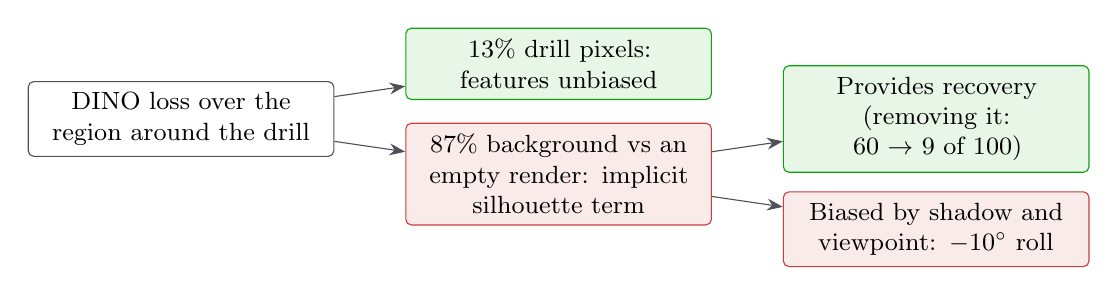
\begin{tikzpicture}[font=\small,node distance=4mm and 9mm,
  bx/.style={draw=inktwo,rounded corners=2pt,align=center,inner sep=4pt,text width=3.6cm},
  ok/.style={bx,fill=good!10,draw=good},
  bad/.style={bx,fill=crit!10,draw=crit},
  ar/.style={-{Stealth[length=2mm]},draw=inktwo}]
\node[bx] (loss) {DINO loss over the\\region around the drill};
\node[ok,right=of loss,yshift=7mm] (obj) {13\% drill pixels:\\features unbiased};
\node[bad,right=of loss,yshift=-7mm] (bg) {87\% background vs an\\empty render: implicit\\silhouette term};
\node[ok,right=of bg,yshift=7mm] (rest) {Provides recovery\\(removing it: 60 $\to$ 9 of 100)};
\node[bad,right=of bg,yshift=-7mm] (bias) {Biased by shadow and\\viewpoint: $-10^\circ$ roll};
\draw[ar] (loss) -- (obj); \draw[ar] (loss) -- (bg);
\draw[ar] (bg) -- (rest); \draw[ar] (bg) -- (bias);
\end{tikzpicture}
\caption{Mechanism of the roll error in our splats. Ground truth was verified exact; the drill's own features have their minimum within $1^\circ$ of the true pose in all 16 views tested. The static $-10^\circ$ offset is not reproduced by the official splat (Section~\ref{sec:official}).}
\end{figure}

\begin{figure}[H]
\centering
\begin{subfigure}[b]{0.49\linewidth}\centering
\includegraphics[width=\linewidth]{\figdir/finding_argmin.pdf}
\caption{Roll at the minimum of the DINO loss, drill at the true pose. The drill-only mask uses ground truth and is a diagnostic only.}
\end{subfigure}\hfill
\begin{subfigure}[b]{0.49\linewidth}\centering
\includegraphics[width=\linewidth]{\figdir/finding_fixes.pdf}
\caption{Corrections tested on the same 100 in-grasp trials.}
\end{subfigure}
\caption{None of the six corrections passes the criterion fixed before the runs (better than POGS in at least two settings, worse in none, and better than a depth-only control). RGB has the highest total but is significantly worse at $+30^\circ$ and raises the roll error by half ($14^\circ$ vs $9.4^\circ$). Each correction fails for a different reason: occlusion by the gripper (depth), changes in shading (RGB), loss of the restoring force (masks), and a stale background once the drill moves (rendered background).}
\end{figure}

\vspace{-2mm}
\paragraph{Also established.}
\begin{itemize}
\item The paper's success rule ignores roll about the bit axis; 94\% of our pre-perturbation rotation error is that roll ($9.5\pm2.8^\circ$).
\item Replacing the DINO backbone (DINOv2 with registers, DINOv3) or upsampling its features (AnyUp) does not remove the bias.
\item The difference between $+$ and $-$ perturbations follows a systematic yaw bias (positive in 83\% of trials). The background treatment changes its sign, but it persists without DINO, so its cause remains open.
\end{itemize}

%==========================================================================
\section{Check with the official POGS code (25 Nov)}\label{sec:official}
We trained and ran the official POGS release on the same simulated capture. Environment deviations: Python 3.10 with a newer torch/CUDA, simulator masks in place of Detic, and a pure-torch stand-in for the hash-grid library of the grouping heads. Every test was written down before it ran.
\begin{table}[H]\centering\small
\begin{tabular}{@{}p{0.62\linewidth}p{0.3\linewidth}@{}}\toprule
Test & Result\\\midrule
Official loss has the $-10^\circ$ roll minimum with the gripper's shadow & not met ($+2^\circ$)\\
Official loss follows the shadow strength & not met ($\rho=0.00$)\\
Official and our loss agree on 13 views without the gripper & met ($\rho=0.53$, median $2^\circ$)\\
Official tracker has the roll error before the gripper touches the drill & met (median $19.4^\circ$; no-motion baseline $0^\circ$)\\
An initialisation on the region around the drill removes it & not met\\
Official tracker on 40 in-grasp trials (paper's rule) & 0/40 (no-motion 0/40; ours 10--24/40)\\\bottomrule
\end{tabular}\end{table}
\textbf{Reading.} Our tracker follows the official tracker's roll during the approach within a median of $0.7^\circ$, so the re-implementation is faithful. The roll error that the paper's rule ignores is real in the official code as well, and larger. Its common cause is a nearly flat, asymmetric roll landscape that the descending gripper tilts towards large negative roll (Fig.~\ref{fig:landscape}); the tracker slides at its step limit. The static, shadow-driven $-10^\circ$ offset of Section~\ref{sec:further} belongs to our splats only: swapping splats between the two pipelines shows the tracking objectives agree and the splats differ.
\begin{figure}[H]\centering
\includegraphics[width=0.9\linewidth]{\figdir/roll_landscape.pdf}
\caption{Roll landscape of the tracking loss at the true pose over the approach, official and our splat. As the gripper descends (frames 2--3) the loss slopes towards large negative roll in both.}\label{fig:landscape}
\end{figure}

%==========================================================================
\section{Next steps and open questions}
\begin{enumerate}
\item Submit an RSS 2027 Stage~1 extended abstract (due 4 Dec) centred on the evaluation finding, now reproduced with the official code; the mechanism is reported with its limits.
\item One pre-registered test of an explicit, shadow-free silhouette term from depth (6 GPU hours, same criterion), if a known gripper model may be used to exclude gripper pixels.
\item Real-data validation with our own captures (drill, AprilTag board, one lamp), or with the authors' data if shared.
\end{enumerate}
\textbf{Questions.} (1) Is a mechanism paper an acceptable outcome, and at which venue? (2) May the tracker use a known gripper model to exclude gripper pixels (POGS lists this as future work)?

\end{document}
